\documentclass[10pt,twocolumn,letterpaper]{article}

\usepackage{cvpr}
\usepackage{times}
\usepackage{epsfig}
\usepackage{graphicx}
\usepackage{amsmath}
\usepackage{amssymb}
\usepackage{hyperref}
\usepackage{listings}
\usepackage{url}
\usepackage{xcolor}
\usepackage{float}

% Code styling
\definecolor{codegreen}{rgb}{0,0.6,0}
\definecolor{codegray}{rgb}{0.5,0.5,0.5}
\definecolor{codepurple}{rgb}{0.58,0,0.82}
\definecolor{backcolour}{rgb}{0.95,0.95,0.92}

\lstdefinestyle{cppstyle}{
    backgroundcolor=\color{backcolour},   
    commentstyle=\color{codegreen},
    keywordstyle=\color{magenta},
    numberstyle=\tiny\color{codegray},
    stringstyle=\color{codepurple},
    basicstyle=\ttfamily\footnotesize,
    breakatwhitespace=false,         
    breaklines=true,                 
    captionpos=b,                    
    keepspaces=true,                 
    numbers=left,                    
    numbersep=5pt,                  
    showspaces=false,                
    showstringspaces=false,
    showtabs=false,                  
    tabsize=2,
    language=C++,
    morekeywords={pragma, omp, parallel, for, simd, schedule, static}
}

\lstset{style=cppstyle}

% Include other packages here, before hyperref.

% If you comment hyperref and then uncomment it, you should delete
% egpaper.aux before re-running latex.  (Or just hit 'q' on the first latex
% run, let it finish, and you should be clear).
%\usepackage[pagebackref=true,breaklinks=true,letterpaper=true,colorlinks,bookmarks=false]{hyperref}

\cvprfinalcopy % *** Uncomment this line for the final submission

\def\cvprPaperID{****} % *** Enter the CVPR Paper ID here
\def\httilde{\mbox{\tt\raisebox{-.5ex}{\symbol{126}}}}

% Pages are numbered in submission mode, and unnumbered in camera-ready
\ifcvprfinal\pagestyle{empty}\fi
\begin{document}

%%%%%%%%% TITLE
\title{BOIDS: Analysis of speedup achieved through parallel programming on CPU}

\author{Gianni Moretti\\
E-mail address\\
{\tt\small gianni.moretti@edu.unifi.it}
% For a paper whose authors are all at the same institution,
% omit the following lines up until the closing ``}''.
% Additional authors and addresses can be added with ``\and'',
% just like the second author.
% To save space, use either the email address or home page, not both
}

\maketitle
\thispagestyle{empty}

%%%%%%%%% ABSTRACT
\begin{abstract}
This project explores the implementation and performance analysis of a Boids simulation in C++ with sequential and OpenMP-parallelized versions. The study compares two data layouts, Array of Structures (AoS) and Structure of Arrays (SoA), to assess their impact on performance.

Results demonstrate significant speedup with parallelization and highlight the importance of data organization for memory access efficiency. The findings underscore the value of combining parallelization and optimized data layouts in high-performance simulations. All the code used on this project can be found on https://github.com/GianniMoretti/Boids.
\end{abstract}

%%%%%%%%% BODY TEXT
\noindent\large\textbf{Future Distribution Permission}\\
\indent The author(s) of this report give permission for this document to be distributed to Unifi-affiliated students taking future courses.

\section{Introduction}
The Boids algorithm, introduced by Craig Reynolds, simulates collective behaviors such as flocking or schooling through simple interaction rules. However, its computational cost grows with the number of agents, making efficient implementations essential for large-scale simulations.
This project investigates the performance optimization of the Boids algorithm using parallel computing with OpenMP. A sequential version was implemented to establish a baseline, while a parallelized version, utilizing the Structure of Arrays (SoA) layout, was developed to exploit multi-core architectures. Additionally, a comparison between Array of Structures (AoS) and SoA was performed in the sequential implementation to analyze the impact of data organization.

\subsection{Understanding the Boids Algorithm}
The Boids algorithm, introduced by Craig Reynolds in 1986, is a model for simulating the flocking behavior of agents such as birds, fish, or other organisms that exhibit group dynamics. Each agent, referred to as a "boid" follows three fundamental rules:

\begin{itemize}
    \item \textbf{Alignment}: A boid aligns its direction with the average heading of its neighbors.  
    \item \textbf{Cohesion}: A boid moves toward the average position of its neighbors to maintain group structure.  
    \item \textbf{Separation}: A boid steers away from nearby neighbors to avoid collisions.  
\end{itemize}

\begin{figure}[H]
\centering
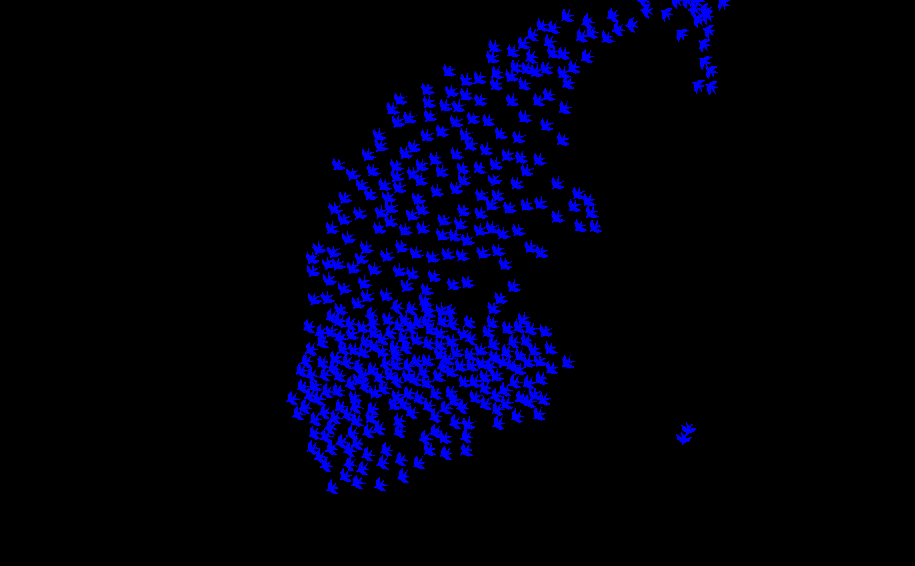
\includegraphics[width=0.8\columnwidth]{../../images/boidsvisualizzationexample.png}
\caption{Visual representation of Boids simulation showing emergent flocking behavior through local interactions.}
\label{fig:boids_visualization}
\end{figure}

These rules are computed independently for each boid at every simulation step, creating emergent behaviors that resemble real-world flocking.  

\subsection{Related Work}
This project is based on the implementation described by \href{https://vanhunteradams.com/Pico/Animal_Movement/Boids-algorithm.html}{Van Hunter Adams}, which provides a concise and efficient version of the algorithm. The implementation organizes the rules into a series of updates on boid positions and velocities, iterated across all agents in the simulation.

By combining these rules, the algorithm achieves realistic collective behaviors without explicit control of the group, highlighting the power of simple local interactions in generating complex global patterns.

\section{Language and Libraries}
The project is implemented in C++ using the OpenMP library for parallelization. OpenMP provides a straightforward way to parallelize loops and sections of code, making it suitable for the Boids algorithm, where each boid's behavior can be computed independently. The choice of C++ allows for efficient memory management and performance optimization, crucial for high-performance simulations.
To visualize the simulation, the project uses the SFML (Simple and Fast Multimedia Library) for rendering the boids on the screen. SFML provides a simple interface for graphics, making it easy to create a visual representation of the simulation.

\section{Methodology}
\subsection{Sequential Implementation}
The sequential implementation of the Boids algorithm serves as the baseline for performance evaluation. In this version, the simulation iteratively updates the state of each boid by applying the three fundamental rules: alignment, cohesion, and separation. Each boid's position and velocity are recalculated at every simulation step based on the states of all other boids.

The main loop processes each boid in sequence, computing the influence of neighboring boids and updating the properties accordingly. Temporary buffers are used to store the new states before copying them back to the main data structures. This approach ensures that updates for one boid do not interfere with the calculations for others within the same iteration.

A representative pseudocode snippet of the update process is provided in the Appendix (see Section~\ref{appendix:seqcode}).

This structure is common to all implementations, with the main differences lying in how data is organized (AoS vs SoA) and whether the outer loop is parallelized. The sequential version provides a clear and straightforward reference for measuring the impact of data layout and parallelization strategies.

\subsection{Data Layouts: AoS vs SoA}
The project implements and compares two distinct data layouts for representing the state of the boids: Array of Structures (AoS) and Structure of Arrays (SoA).

In the \textbf{AoS} approach, each boid is represented as a structure containing all its properties (position, velocity, bias, etc.), and a vector of these structures is used to store the entire flock. This is reflected in the following structure:
\begin{lstlisting}[language=C++]
struct BoidData {
    sf::Vector2f position;
    sf::Vector2f velocity;
    float biasval;
    int scoutGroup;
    // ...
};
std::vector<BoidData> boidDataList;
\end{lstlisting}
With this layout, the main loop iterates over the vector, and each boid's state is accessed as a whole. This approach is intuitive and convenient for object-oriented programming, but can lead to less efficient memory access patterns, especially when only a subset of fields is needed for computation.

In the \textbf{SoA} approach, each property of the boids is stored in a separate array. For example, all positions are stored in one array, all velocities in another, and so on. The structure is defined as:
\begin{lstlisting}[language=C++]
struct BoidDataList {
    float* xPos;
    float* yPos;
    float* xVelocity;
    float* yVelocity;
    float* biasvals;
    int* scoutGroup;
    int numBoid;
    // ...
};
\end{lstlisting}
This layout enables more efficient memory access, particularly when performing operations over a single property for all boids. In the main loop, the SoA version processes each property in bulk, which improves cache utilization and can be more easily vectorized by the compiler.

\textbf{Key differences in computation:}
In the AoS version, the main loop iterates over the vector of structures, accessing and updating each boid's fields individually. In the SoA version, the main loop operates over arrays of properties, often using local variables to accumulate results before writing back to the arrays. The SoA layout allows for better spatial locality and enables optimizations such as SIMD vectorization, as memory accesses are more predictable and contiguous.

\textbf{Performance advantages of SoA:}
The SoA approach provides improved cache efficiency when accessing the same property across many boids, reduced memory bandwidth usage due to contiguous memory access patterns, and easier application of parallelization and vectorization techniques.

A detailed example of the data structures and main loop implementations for both layouts is provided in the Appendix (see Section~\ref{appendix:aossoa}).

\subsection{Parallel Implementation}
The parallel implementation is based on the SoA (Structure of Arrays) version, as this layout is more suitable for parallel and vectorized operations. The main goal of the parallelization is to distribute the computation of each boid's behavior across multiple CPU threads using OpenMP.

The core idea is that the update of each boid at each simulation step is independent from the others, as all computations are based on the current state and do not interfere with updates of other boids. This makes the outer loop over boids a natural candidate for parallelization.

In the parallel version, several key changes were introduced. The main update loop over all boids is annotated with \texttt{\#pragma omp parallel for}, allowing OpenMP to assign different iterations (boids) to different threads. Each thread works with its own set of local variables for the computation of new positions, velocities, and bias values, avoiding race conditions. Temporary arrays are allocated to store the updated properties for all boids. After the parallel loop, these arrays are copied back to the main SoA structure in a separate loop, which can also be vectorized (e.g., with \texttt{\#pragma omp simd}). The number of threads can be configured at runtime, and OpenMP automatically manages the workload distribution.

This approach ensures that all memory accesses within the parallel region are thread-safe, as each thread writes to a unique index in the temporary arrays. The SoA layout further improves performance by enabling contiguous memory access and better cache utilization.

A simplified example of the parallelized loop is provided in the Appendix (see Section~\ref{appendix:parloop}).

\section{Results and Discussion}

Performance evaluation was conducted across varying numbers of boids and thread configurations to assess the scalability and computational efficiency of different implementations. The testing methodology compared the sequential AoS implementation against the parallel SoA version using OpenMP.

\subsection{Testing Environment and Methodology}
All benchmarks were conducted on a system with multiple CPU cores using identical simulation parameters. The evaluation focused on execution time measurements across different boid populations (1,000 to 32,000 boids) and thread counts (1 to 12 threads) to analyze both sequential performance and parallel scalability. The benchmark methodology involved fixed simulation parameters across all tests to ensure consistency, multiple runs per configuration to compute statistical averages, and isolated measurement of the main simulation loop to exclude rendering overhead.

\subsection{AoS vs SoA Performance Comparison}

\begin{figure*}[t]
\centering
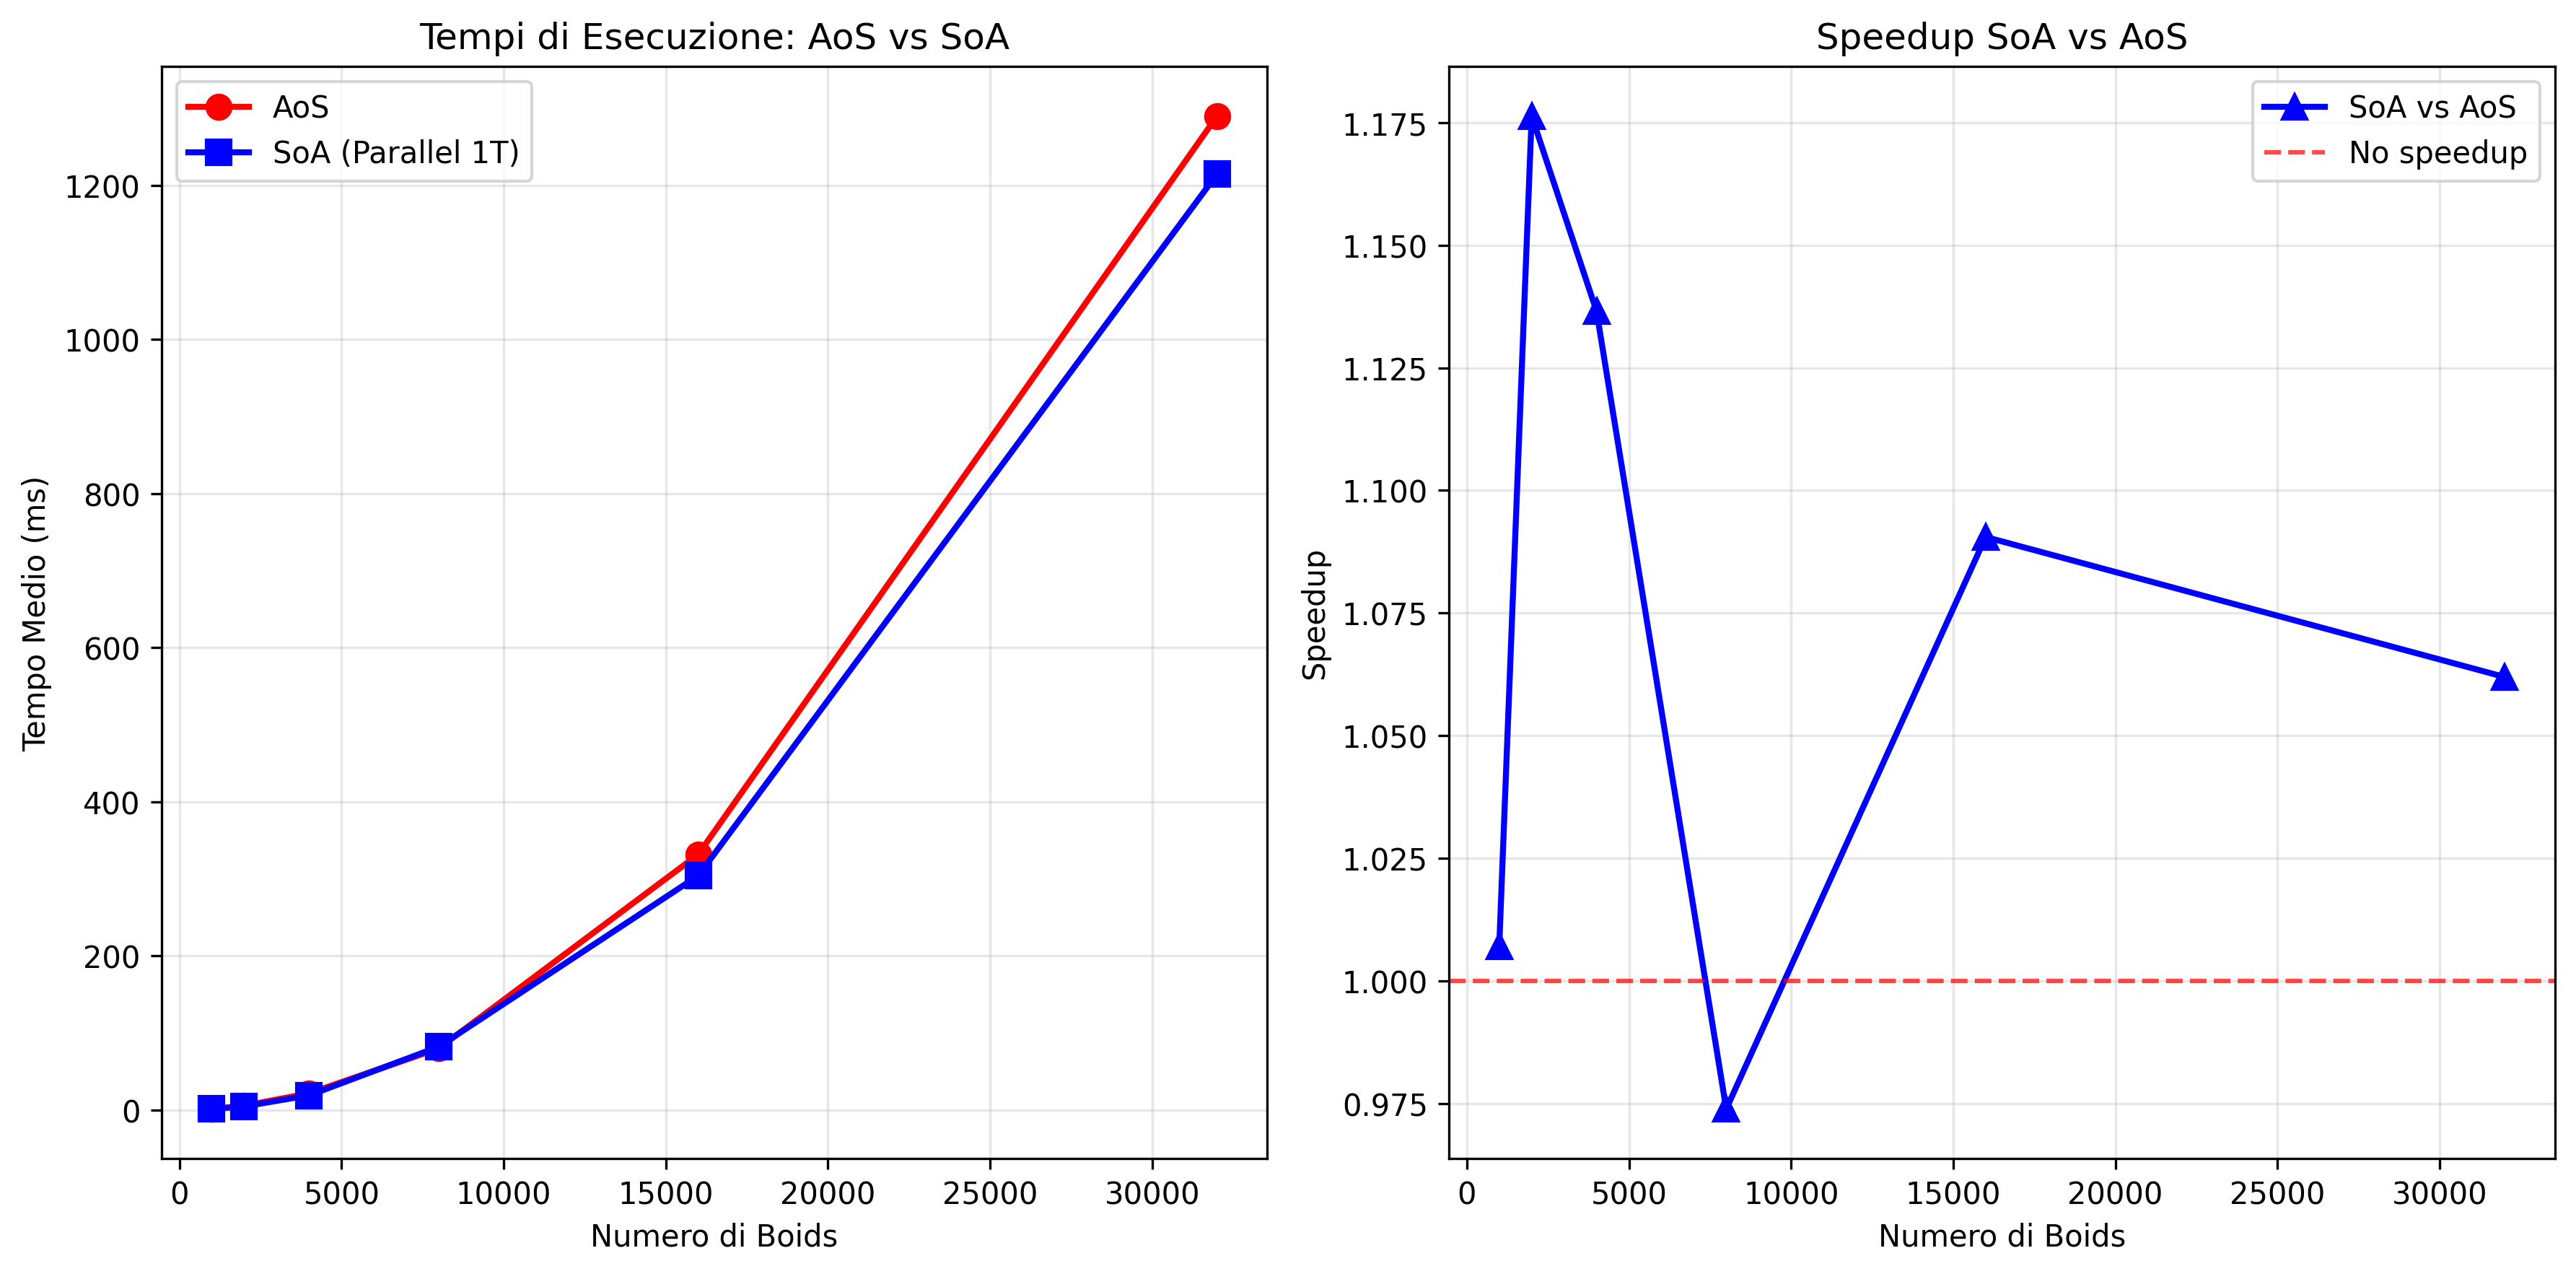
\includegraphics[width=0.8\textwidth]{../../images/aos_vs_soa.png}
\caption{Performance comparison between Array of Structures (AoS) and Structure of Arrays (SoA) implementations showing the impact of data layout on execution time.}
\label{fig:aos_vs_soa}
\end{figure*}

The comparison between AoS and SoA data layouts reveals modest performance differences based on the benchmark results. The SoA layout (represented by the "Parallel" implementation with 1 thread) demonstrates slightly superior performance characteristics compared to AoS across most tested configurations. For 1,000 boids, AoS required 1.43ms while SoA achieved 1.42ms, showing essentially equivalent performance. The performance gap becomes more noticeable with larger datasets: at 32,000 boids, AoS required 1,290.09ms compared to 1,214.82ms for SoA, representing a modest 6.2\% improvement.

While the SoA layout enables better cache utilization through contiguous memory access when processing the same property across multiple boids, in this specific implementation the performance advantage is relatively small. This suggests that for the Boids algorithm, the benefits of improved spatial locality and reduced memory bandwidth usage are present but not as pronounced as in other types of computations that might benefit more dramatically from vectorization and cache optimization.

\subsection{Parallel Speedup Analysis}

\begin{figure*}[t]
\centering
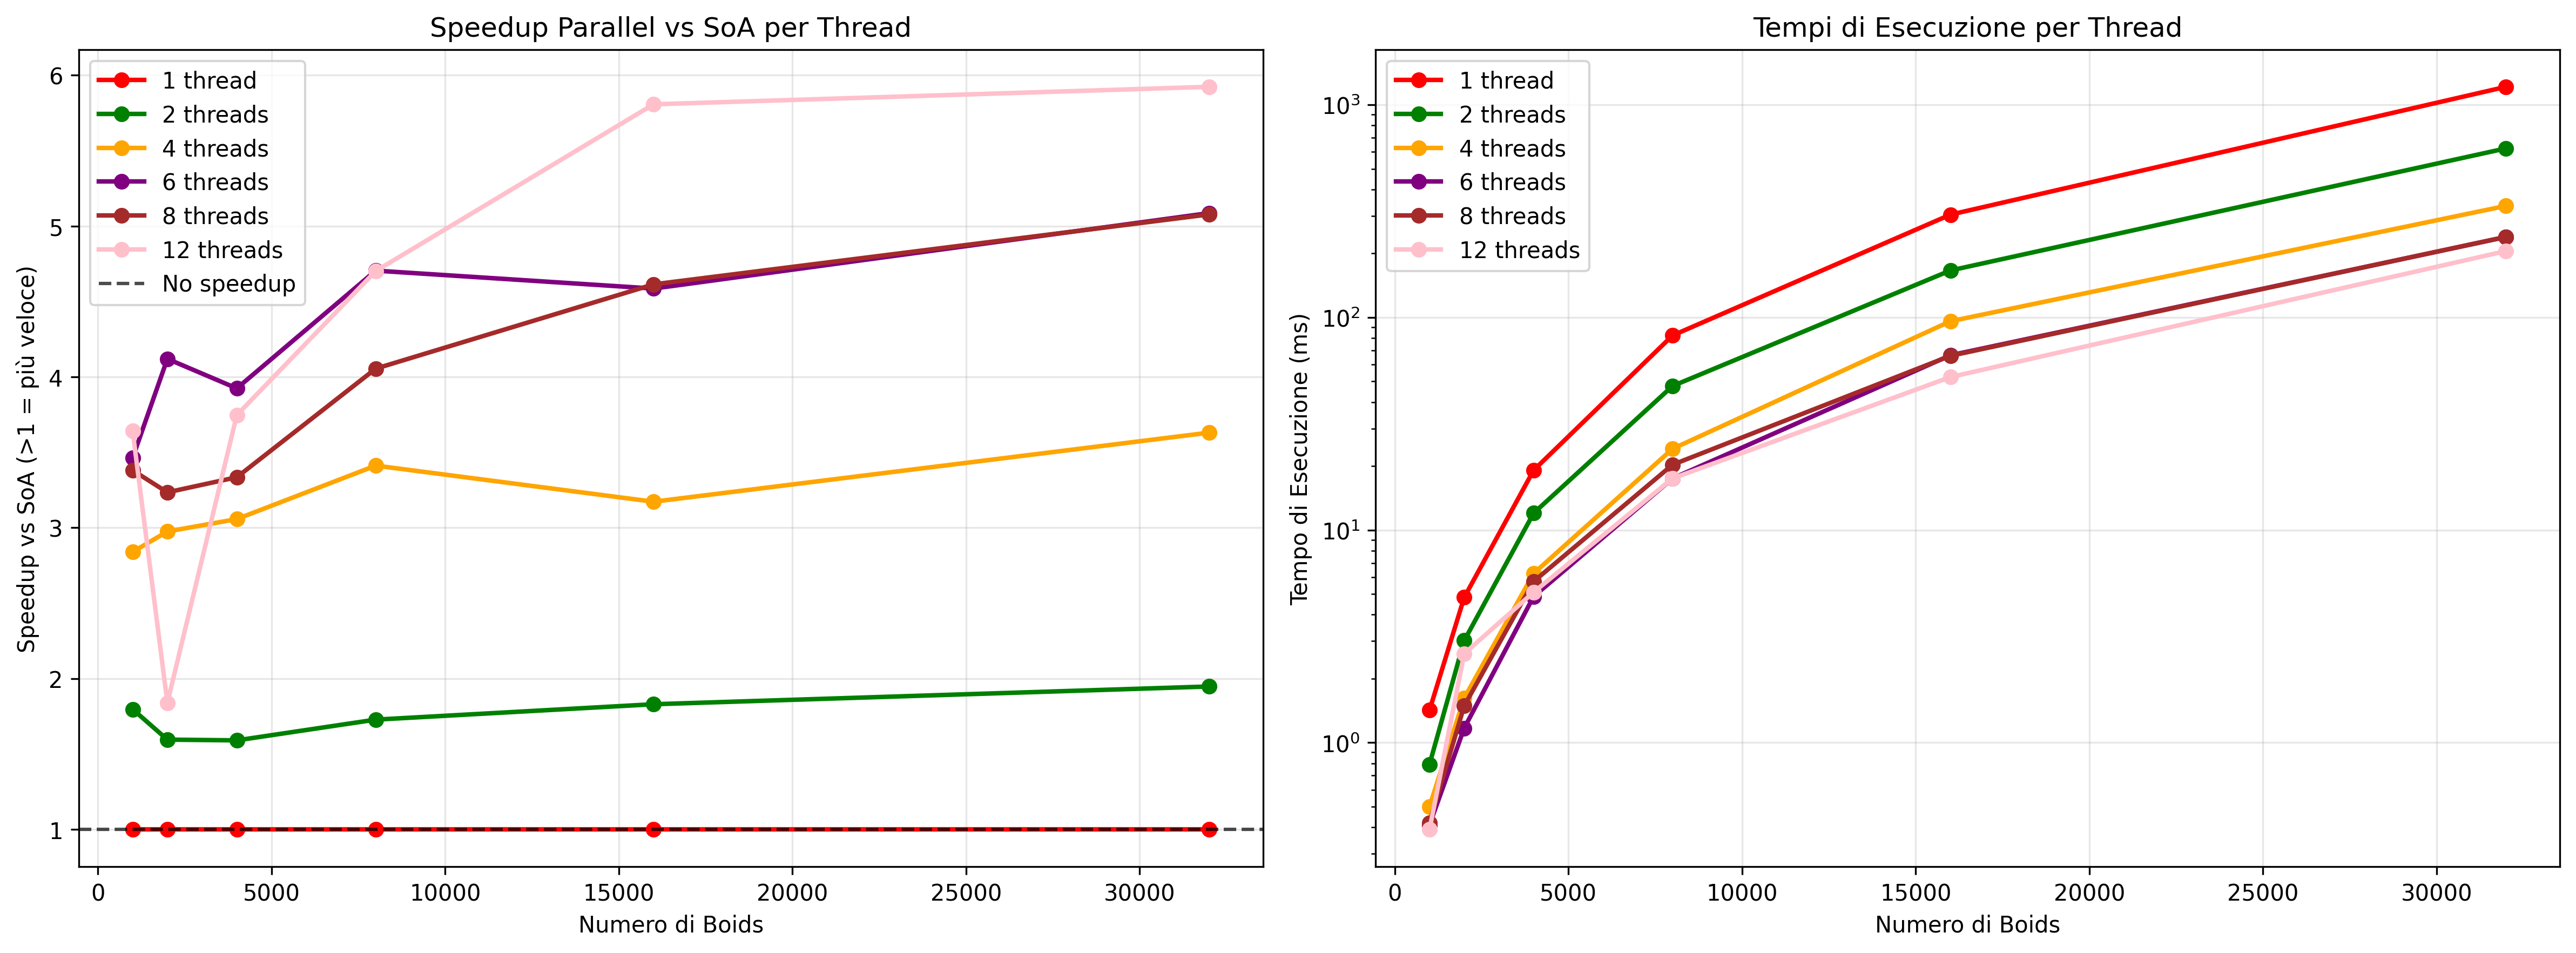
\includegraphics[width=0.8\textwidth]{../../images/parallel_analysis_performance.png}
\caption{Execution time analysis showing performance across different numbers of boids and thread configurations.}
\label{fig:performance_analysis}
\end{figure*}

\begin{figure*}[t]
\centering
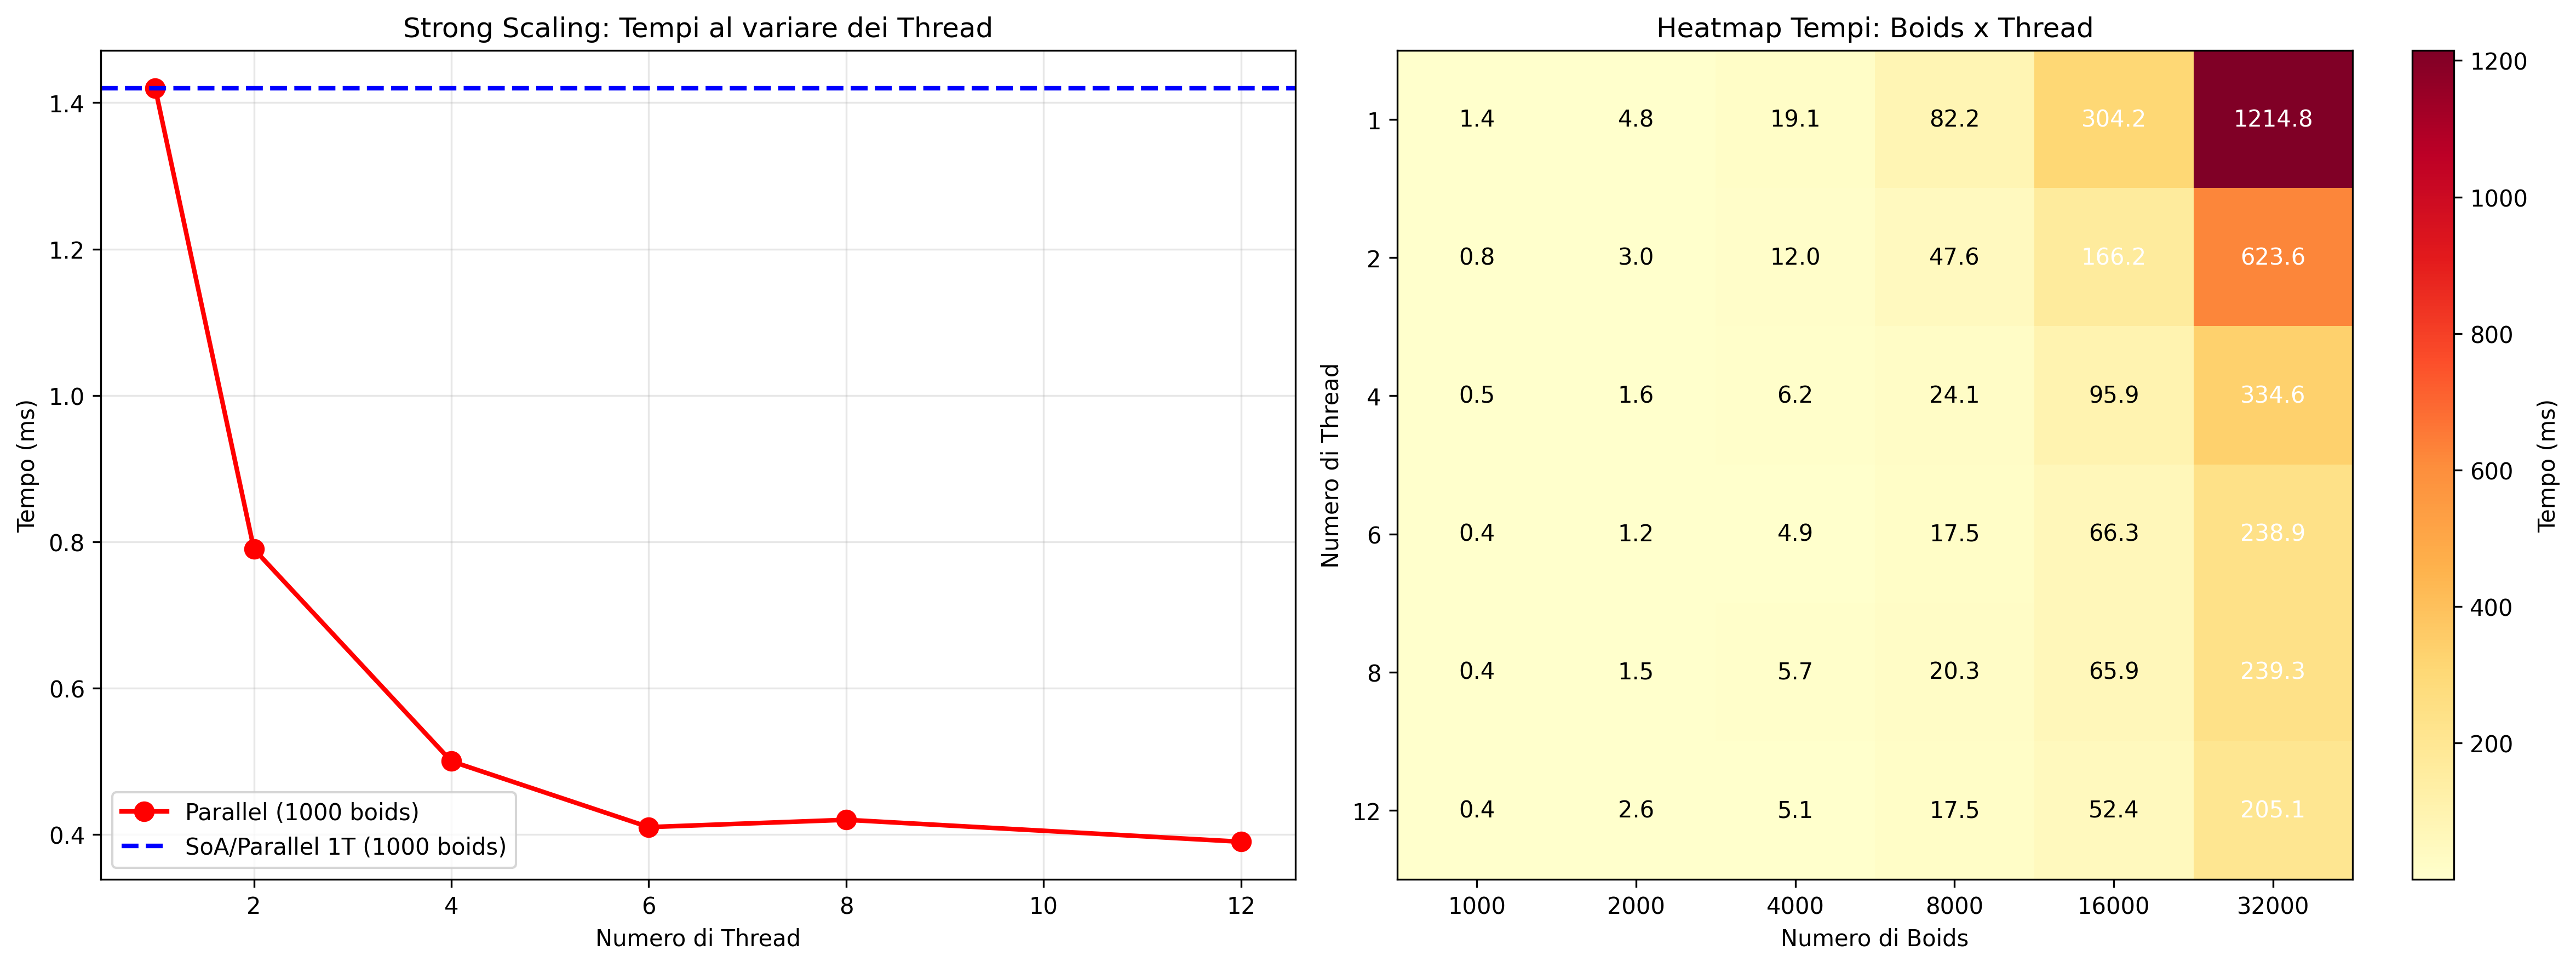
\includegraphics[width=0.8\textwidth]{../../images/parallel_analysis_scaling.png}
\caption{Parallel scaling efficiency demonstrating speedup characteristics with increasing thread count.}
\label{fig:scaling_analysis}
\end{figure*}

The parallel implementation using OpenMP demonstrates significant performance improvements across all tested configurations. The benchmark data reveals optimal thread configurations vary with dataset size:

For 1,000 boids, the best performance is achieved with 12 threads at 0.39ms, representing a 3.6x speedup compared to sequential execution (1.42ms). The performance scaling shows near-linear improvement from 1 to 6 threads, with diminishing returns beyond 8 threads.

For larger datasets, the optimal thread count stabilizes around 6-12 threads. With 32,000 boids, 12 threads achieve 205.12ms compared to 1,214.82ms sequential, delivering a 5.9x speedup. The 6-thread configuration achieves 238.88ms (5.1x speedup), demonstrating that significant performance gains are achievable even with moderate thread counts.

The parallel implementation successfully mitigates the O(N²) computational complexity inherent in the Boids algorithm. The scaling behavior shows consistent improvements across all dataset sizes, with the most significant gains observed in the 4-12 thread range where the balance between parallelization benefits and overhead costs is optimal.

\section{Conclusion}

This project successfully demonstrates the significant impact of parallel programming techniques and optimized data layouts on the performance of computationally intensive simulations. The comprehensive analysis of the Boids algorithm implementation reveals several key findings that extend beyond the specific application to broader principles of high-performance computing.

\subsection{Key Achievements}

The parallel implementation using OpenMP achieved substantial performance improvements, with speedups ranging from 2.5x to 5.9x compared to sequential execution. These results validate the effectiveness of the chosen parallelization strategy and demonstrate the practical benefits of leveraging multi-core architectures for embarrassingly parallel problems.

The comparison between AoS and SoA data layouts revealed modest performance differences, with SoA providing slightly better cache utilization and memory access patterns in this specific implementation. While the theoretical advantages of SoA are well-established, in this particular case the performance gain was limited to approximately 6.2\% for the largest dataset, demonstrating that the impact of data structure optimization can vary significantly depending on the specific algorithm and access patterns.

\subsection{Implications for High-Performance Computing}

Several broader implications emerge from this work. Data layout optimization represents a fundamental trade-off in computational efficiency, with SoA generally favoring operations that process the same property across multiple entities. The observed performance characteristics highlight the importance of finding the optimal balance between parallelization benefits and overhead costs. Cache-friendly data access patterns significantly impact performance, particularly for memory-bound algorithms.

\subsection{Broader Impact}

The methodologies and insights developed in this project are applicable to a wide range of computational problems beyond Boids simulation, including particle systems in physics simulations, agent-based modeling in social sciences and economics, molecular dynamics simulations in computational chemistry, and computer graphics and game development applications.

The project successfully demonstrates that careful consideration of data structures, memory access patterns, and parallelization strategies can yield substantial performance improvements, making complex simulations feasible on standard multi-core hardware. These findings contribute to the broader understanding of high-performance computing principles and their practical application in scientific and engineering contexts.

%%%%%%%%% REFERENCES
{\small
\begin{thebibliography}{99}

\bibitem{reynolds}
Craig W. Reynolds.
\textit{Flocks, herds and schools: A distributed behavioral model}.
SIGGRAPH '87: Proceedings of the 14th Annual Conference on Computer Graphics and Interactive Techniques, 1987.

\bibitem{vanhunter}
Van Hunter Adams.
\textit{Boids Algorithm Implementation}.
\url{https://vanhunteradams.com/Pico/Animal_Movement/Boids-algorithm.html}, 2024.

\bibitem{openmp}
OpenMP Architecture Review Board.
\textit{OpenMP Application Programming Interface Specification}.
Version 5.2, 2021.

\bibitem{sfml}
Laurent Gomila et al.
\textit{SFML - Simple and Fast Multimedia Library}.
\url{https://www.sfml-dev.org/}, 2024.

\bibitem{bertini}
Marco Bertini.
\textit{Parallel Computing Course Lectures}.
Department of Information Engineering, University of Florence, 2024.

\end{thebibliography}
}

\appendix
\section*{Appendix}
\addcontentsline{toc}{section}{Appendix}

\subsection*{Sequential Update Loop Example}
\label{appendix:seqcode}
\begin{lstlisting}[language=C++, caption=Sequential Boids update loop structure]
for (int i = 0; i < num_boids; i++) {
    float alignment_x = 0, alignment_y = 0;
    float cohesion_x = 0, cohesion_y = 0;
    float separation_x = 0, separation_y = 0;
    int neighbor_count = 0;
    
    for (int j = 0; j < num_boids; j++) {
        if (i != j) {
            float dx = boids[j].x - boids[i].x;
            float dy = boids[j].y - boids[i].y;
            float distance = sqrt(dx*dx + dy*dy);
            
            if (distance < perception_radius) {
                // Apply alignment, cohesion, separation rules
                alignment_x += boids[j].vx;
                alignment_y += boids[j].vy;
                cohesion_x += boids[j].x;
                cohesion_y += boids[j].y;
                // ... separation logic
                neighbor_count++;
            }
        }
    }
    // Update velocity and position based on computed forces
    boids[i].vx += (alignment_x + cohesion_x + separation_x);
    boids[i].vy += (alignment_y + cohesion_y + separation_y);
    boids[i].x += boids[i].vx * dt;
    boids[i].y += boids[i].vy * dt;
}
\end{lstlisting}

\subsection*{AoS vs SoA Data Structures and Main Loop}
\label{appendix:aossoa}

\textbf{Array of Structures (AoS) Implementation:}
\begin{lstlisting}[language=C++, caption=AoS data structure and main loop]
// Structure definition
struct BoidData {
    sf::Vector2f position;
    sf::Vector2f velocity;
    float biasval;
    int scoutGroup;
    sf::Color color;
};

std::vector<BoidData> boidDataList;

// Main loop implementation
for (int i = 0; i < boidDataList.size(); i++) {
    BoidData refBoid = boidDataList[i];
    sf::Vector2f alignment(0, 0);
    sf::Vector2f cohesion(0, 0);
    sf::Vector2f separation(0, 0);
    
    // Compute interactions with all other boids
    for (int j = 0; j < boidDataList.size(); j++) {
        if (i != j) {
            sf::Vector2f diff = boidDataList[j].position - refBoid.position;
            float distance = sqrt(diff.x * diff.x + diff.y * diff.y);
            
            if (distance < perceptionRadius) {
                alignment += boidDataList[j].velocity;
                cohesion += boidDataList[j].position;
                // ... separation and other rule calculations
            }
        }
    }
    
    // Apply computed forces and update boid
    refBoid.velocity += alignment + cohesion + separation;
    refBoid.position += refBoid.velocity * deltaTime;
    boidDataList_tmp.emplace_back(refBoid);
}
boidDataList = boidDataList_tmp;
\end{lstlisting}

\textbf{Structure of Arrays (SoA) Implementation:}
\begin{lstlisting}[language=C++, caption=SoA data structure and main loop]
// Structure definition
struct BoidDataList {
    float* xPos;
    float* yPos;
    float* xVelocity;
    float* yVelocity;
    float* biasvals;
    int* scoutGroup;
    int numBoid;
    
    // Constructor allocates contiguous memory arrays
    BoidDataList(int n) : numBoid(n) {
        xPos = new float[n];
        yPos = new float[n];
        xVelocity = new float[n];
        yVelocity = new float[n];
        biasvals = new float[n];
        scoutGroup = new int[n];
    }
};

// Main loop implementation
for (int i = 0; i < N; i++) {
    float tmp_pos_x = xPos[i];
    float tmp_pos_y = yPos[i];
    float tmp_vel_x = xVelocity[i];
    float tmp_vel_y = yVelocity[i];
    
    float alignment_x = 0, alignment_y = 0;
    float cohesion_x = 0, cohesion_y = 0;
    float separation_x = 0, separation_y = 0;
    
    // Process neighbors using array accesses
    for (int j = 0; j < N; j++) {
        if (i != j) {
            float dx = xPos[j] - tmp_pos_x;
            float dy = yPos[j] - tmp_pos_y;
            float distance = sqrt(dx*dx + dy*dy);
            
            if (distance < perceptionRadius) {
                alignment_x += xVelocity[j];
                alignment_y += yVelocity[j];
                cohesion_x += xPos[j];
                cohesion_y += yPos[j];
                // ... separation calculations
            }
        }
    }
    
    // Update arrays with new values
    new_xVelocity[i] = tmp_vel_x + alignment_x + cohesion_x + separation_x;
    new_yVelocity[i] = tmp_vel_y + alignment_y + cohesion_y + separation_y;
    new_xPos[i] = tmp_pos_x + new_xVelocity[i] * deltaTime;
    new_yPos[i] = tmp_pos_y + new_yVelocity[i] * deltaTime;
}

// Copy results back to main arrays
std::memcpy(xPos, new_xPos, N * sizeof(float));
std::memcpy(yPos, new_yPos, N * sizeof(float));
std::memcpy(xVelocity, new_xVelocity, N * sizeof(float));
std::memcpy(yVelocity, new_yVelocity, N * sizeof(float));
\end{lstlisting}

\subsection*{Parallel SoA Implementation with OpenMP}
\label{appendix:parloop}
\begin{lstlisting}[language=C++, caption=Parallel Boids implementation using OpenMP]
// Allocate temporary arrays for thread-safe updates
float* new_xPos = new float[N];
float* new_yPos = new float[N];
float* new_xVelocity = new float[N];
float* new_yVelocity = new float[N];
float* new_biasvals = new float[N];

// Parallel update loop using OpenMP
#pragma omp parallel for schedule(static) num_threads(num_threads)
for (int i = 0; i < N; i++) {
    // Read current state from SoA arrays (read-only access)
    float tmp_pos_x = xPos[i];
    float tmp_pos_y = yPos[i];
    float tmp_vel_x = xVelocity[i];
    float tmp_vel_y = yVelocity[i];
    float tmp_bias = biasvals[i];
    
    // Local variables for computing forces (thread-private)
    float alignment_x = 0.0f, alignment_y = 0.0f;
    float cohesion_x = 0.0f, cohesion_y = 0.0f;
    float separation_x = 0.0f, separation_y = 0.0f;
    int neighbor_count = 0;
    
    // Evaluate interactions with all other boids
    for (int j = 0; j < N; j++) {
        if (i != j) {
            float dx = xPos[j] - tmp_pos_x;
            float dy = yPos[j] - tmp_pos_y;
            float distance = sqrt(dx*dx + dy*dy);
            
            if (distance < perceptionRadius && distance > 0.0f) {
                float inv_distance = 1.0f / distance;
                
                // Alignment: steer towards average heading of neighbors
                alignment_x += xVelocity[j];
                alignment_y += yVelocity[j];
                
                // Cohesion: steer towards average position of neighbors
                cohesion_x += xPos[j];
                cohesion_y += yPos[j];
                
                // Separation: steer away from close neighbors
                if (distance < separationRadius) {
                    separation_x -= dx * inv_distance;
                    separation_y -= dy * inv_distance;
                }
                
                neighbor_count++;
            }
        }
    }
    
    // Normalize and apply forces if neighbors exist
    if (neighbor_count > 0) {
        float inv_neighbors = 1.0f / neighbor_count;
        alignment_x *= inv_neighbors * alignmentStrength;
        alignment_y *= inv_neighbors * alignmentStrength;
        cohesion_x = (cohesion_x * inv_neighbors - tmp_pos_x) * cohesionStrength;
        cohesion_y = (cohesion_y * inv_neighbors - tmp_pos_y) * cohesionStrength;
        separation_x *= separationStrength;
        separation_y *= separationStrength;
    }
    
    // Update velocity with computed forces
    float new_vel_x = tmp_vel_x + alignment_x + cohesion_x + separation_x;
    float new_vel_y = tmp_vel_y + alignment_y + cohesion_y + separation_y;
    
    // Apply speed limiting
    float speed = sqrt(new_vel_x*new_vel_x + new_vel_y*new_vel_y);
    if (speed > maxSpeed) {
        float scale = maxSpeed / speed;
        new_vel_x *= scale;
        new_vel_y *= scale;
    }
    
    // Store results in temporary arrays (thread-safe writes)
    new_xPos[i] = tmp_pos_x + new_vel_x * deltaTime;
    new_yPos[i] = tmp_pos_y + new_vel_y * deltaTime;
    new_xVelocity[i] = new_vel_x;
    new_yVelocity[i] = new_vel_y;
    new_biasvals[i] = tmp_bias; // bias update logic omitted for brevity
}

// Copy results back to main arrays (can be vectorized)
#pragma omp simd
for (int i = 0; i < N; i++) {
    xPos[i] = new_xPos[i];
    yPos[i] = new_yPos[i];
    xVelocity[i] = new_xVelocity[i];
    yVelocity[i] = new_yVelocity[i];
    biasvals[i] = new_biasvals[i];
}

// Cleanup temporary arrays
delete[] new_xPos;
delete[] new_yPos;
delete[] new_xVelocity;
delete[] new_yVelocity;
delete[] new_biasvals;
\end{lstlisting}

% Additional implementation details or formulas.

%-------------------------------------------------------------------------
\end{document}
